\chapter{Background experimental studies}\label{sec:studies-experiments}

Many experiments were carried out on individual ceramic pebbles. While there are some measures from experiments that are immediately useful for qualitative comparisons, such as the crush strength between different batches of ceramics, most values are not obviously connected to analysis of the pebbles nor the pebble bed assemblies they make up. In this section we will show had careful examination of single pebble experiments can lead to predictions of not only strength in ensembles but also modifications of the fundamental properties of the ceramic pebbles.

In section \cref{sec:exp-reduction-factor}, we use single pebble experiments to validate the use of Hertz theory for contacting ceramic pebbles, but also determine the proper Young's modulus to use for the ceramics. In section \cref{sec:theoryStrainEnergy} we use the theory along with experimental data to begin to make predictions for survivability of pebbles in ensembles.


\subsection{Elasticity Reduction Factor}\label{sec:exp-reduction-factor}

% the following was from the MOTIVATION section of SOFT-2014~~~~~~~~~~~~~~~~~~~~~~
% In the study of individual pebble crush force, the force-travel response curves of ceramic materials consistently exhibit distributions in the stiffness of the pebbles. For example, see the results of different lithium ceramic pebbles in Fig.~\ref{fig:force-travel-exp}. For DEM studies, we claim that interaction between these pebbles is well-represented by the Hertzian normal force as derived in \cref{sec:hertz-theory}. For the discussion, we rewrite Eq.~\ref{eq:hertz-normal-force} here,


% \begin{equation*}
%   F_{n,ij} = \frac{4}{3}E_{ij}^* \sqrt{R_{ij}^*} \, \delta_{n,ij}^{3/2}
% \end{equation*}

% where $\delta$ is the overlap between contacting spheres and $\frac{1}{E^*} = \frac{1-\nu_i^2}{E_i} + \frac{1-\nu_j^2}{E_j}$, $\frac{1}{R^*} = \frac{1}{R_i} + \frac{1}{R_j}$

% From Eq.~\ref{eq:hertz-normal-force}, we see the contact force is directly proportional to the pair Young's modulus, $E^*$. Thus an accurate value of pebble Young's modulus is critical for an accurate calculation of contact force. We now present Hertz equation as it applies to a pebble, diameter of $d_p$, being pressed between two flat anvils with measured travel of one anvil as $s$:

% \begin{equation}\label{eq:peb-anvil-contact-force}
%   F_n = \frac{1}{3}E^*\sqrt{d_ps^3}
% \end{equation} 

% and $\frac{1}{E^*} = \frac{1-\nu_p^2}{E_p} + \frac{1-\nu_a^2}{E_a}$. Where the subscript $p$ refers to pebbles and $a$ the anvils.

% From Eq.~\ref{eq:peb-anvil-contact-force}, we see that standard Hertz theory, where we use a single value for Young's modulus from literature, is not appropriate for pebbles studied in ceramic breeders. If single values of $E_p$ and $\nu_p$ are employed, then variation in pebble diameters can not alone explain the variation of curves of Fig.~\ref{fig:force-travel-exp}.
% %~~~~~~~~~~~~~~~~~~~~~~~~~~~~~~~~~~~~~~~~~~~~~~~~~~~~~~~~~~~~~~~



% \subsubsection{Elasticity reduction factor}
% We propose to explain the behavior of individual pebbles (as in Fig.~\ref{fig:force-travel-exp}) with an assumption that the production technique yields pebbles with slightly different internal structures. The differences in internal structure then cause the pebble to have a different apparent modulus of elasticity; which will vary from some strong limit value. The strong value is the elastic modulus of highly sintered pellets reported in literature for the material, $E_\text{bulk}$. Assuming this strong value is the upper limit, imperfections in the pebbles will lead only to a reduction in this value. To quantify the deviation from the bulk, we introduce a $k$ factor, defined as the elasticity reduction factor:

% \begin{equation}
%   k = \frac{E_\text{peb}}{E_\text{bulk}}
% \end{equation}
% where $k \in [0,1]$.

% If each pebble has a unique $k$ value, this would quantify the spread in elastic responses seen in the experiments. The value is found by assuming that the pebbles are, in fact, behaving in a Hertzian manner, allowing us to back-out its $k$ value, or in other words the unique $E^*$ of that pebble by finding a best fit to the experimental curves. 

% From room temperature, we take the sintered pebble value for these Li$_4$SiO$_4$ pebbles to be $E_\text{bulk} = 90$~GPa and $E_\text{bulk} = 124$~GPa for Li$_4$SiO$_4$ pebbles. Then we iterate over all values of $k\in[0,1]$ and compare the Hertzian response to that pebble's force-displacement curve.

% The data of Fig.~\ref{fig:nfri-force-travel-exp} is fit in the manner described and the pebbles are all plotted against Hertzian curves with their own unique modified Young's modulus in Fig.~\ref{fig:hertz-exp}. The modified Hertzian curves with apparent Young's modulus fits well with most of the pebbles' curves. Similar data is obtained for the pebbles of Fig.~\ref{fig:fzk-force-travel-exp} but the results are omitted for conciseness.


% \begin{figure}
%        \centering
%        \begin{subfigure}[b]{0.45\textwidth}
%                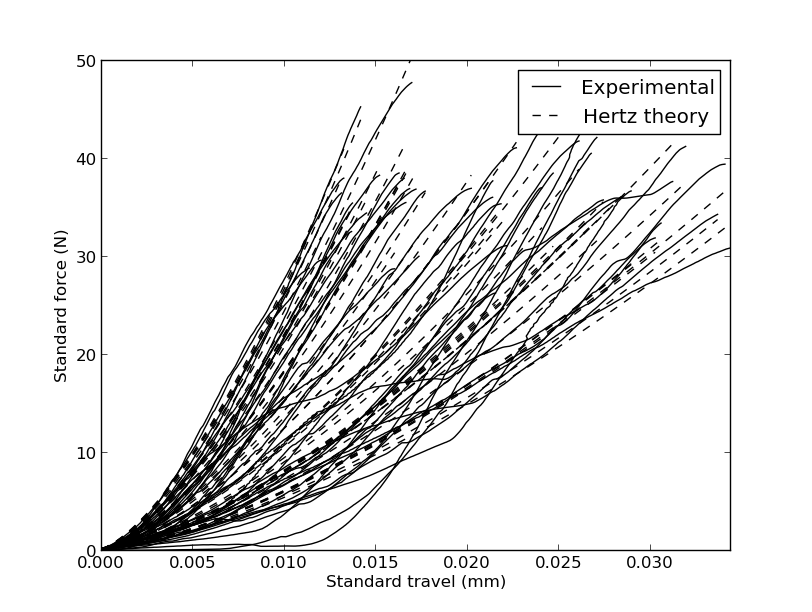
\includegraphics[width=\textwidth]{chapters/figures/NFRI-exp_v_hertz}
%                \caption{Experimental responses (solid) and fit curves of Hertzian equivalent with apparent Young's modulus (dashed).}
%                \label{fig:hertz-exp}
%        \end{subfigure}%
       
%         %add desired spacing between images, e. g. ~, \quad, \qquad, \hfill etc.
%          %(or a blank line to force the subfigure onto a new line)
%        \begin{subfigure}[b]{0.45\textwidth}
%                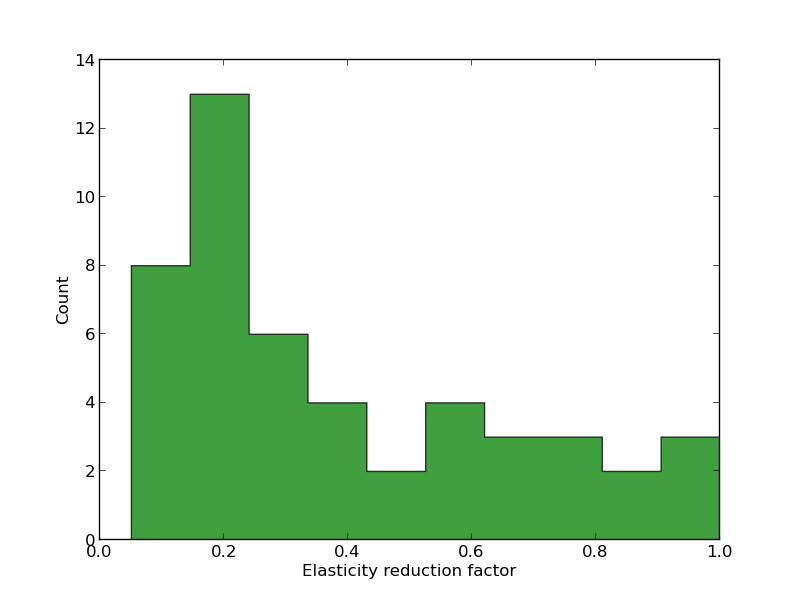
\includegraphics[width=\textwidth]{chapters/figures/NFRI-k_hist}
%                \caption{Distribution of elasticity reduction value, $k$, for the pebbles in this batch of lithium metatitanate. This distribution is modeled as a Weibull distribution function in DEM simulations.}
%                \label{fig:k-hist}
%        \end{subfigure}
%        \caption{An apparent Young's modulus is found for each pebble and the distribution of reduction factor, $k$, shows the quantity of reduction of the stiffness of the pebbles from the value found in literature.}
% \label{fig:hertz-results}
% \end{figure}




% \begin{figure}[t]
% \centering
% 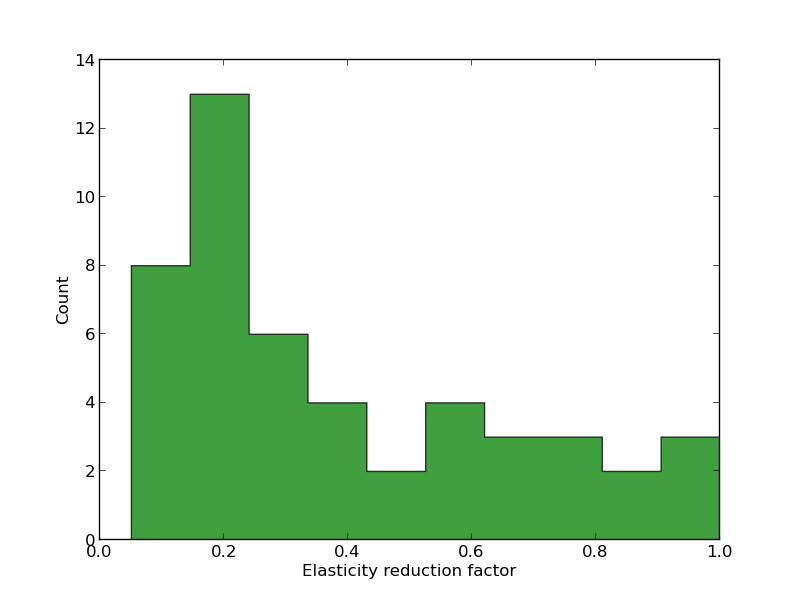
\includegraphics[width = 0.45 \textwidth]{chapters/figures/NFRI-k_hist}
% \caption{Distribution of elasticity reduction value, $k$, for the pebbles in this batch of lithium metatitanate. This distribution is modeled as a Weibull distribution function in DEM simulations.}\label{fig:k-hist}
% \end{figure}

% From the distribution of $k$, we see that the Young's modulus of many of the pebbles is about 20\% of the value of the sintered pellet that is given as the material property from literature. The Hertz contact force for these soft pebbles is then likewise 20\% of the value one would predict if using the Young's modulus from literature! 
% One of the benefits of using DEM simulations is the ability to predict pebble cracking in an ensemble based on knowledge of the interaction forces. If we are over-predicting the contact forces based on inaccurate material properties, we are going to be over-predicting the impact of pebble cracking as well. An accurate description of the material properties is an important feature for ceramic breeder designers.

% We will apply the modified Young's modulus distributions to pebble beds and compare the results to pebble beds simulated with standard Young's modulus from literature.

% \begin{figure}[t]
%   \centering
%   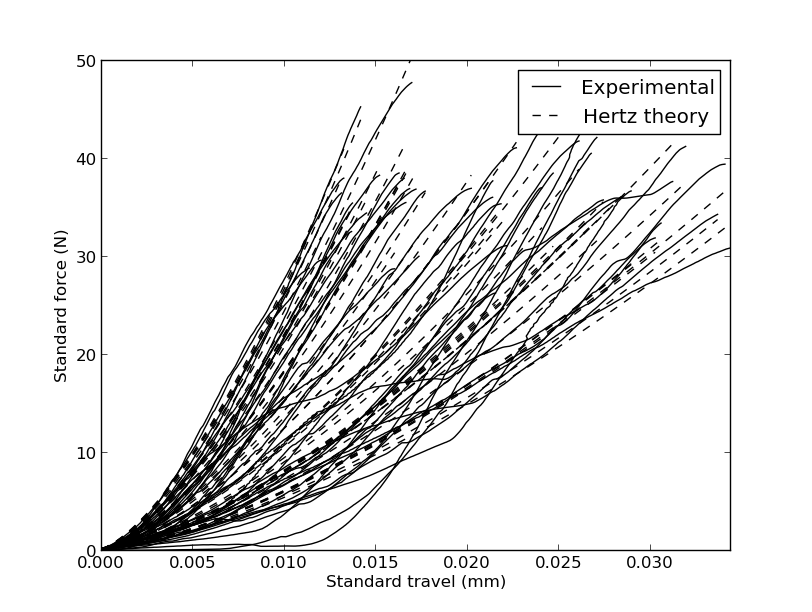
\includegraphics[width = \singleimagewidth]{chapters/figures/NFRI-exp_v_hertz}
%   \caption{Experimental responses (solid) and fit curves of Hertzian equivalent with apparent Young's modulus (dashed).}\label{fig:hertz-exp}
% \end{figure}

%end of the section taken from SOFT 2014 ~~~~~~~~~~~~~~~~~~~~~~~~~~~~~~~~





We introduced Hertz theory in \cref{sec:hertz-theory}, and in \cref{sec:modeling-dem} showed how we apply the Hertzian contact rules into the discrete element computational framework. We will revisit the Hertzian equations as we analyze the force-displacement measurements of single pebbles in the anvils of our uniaxial compression test stand.

The derivation to the Hertz force can be found on page~\pageref{eq:hertz-normal-force} but the result is given again here for reference:
\begin{equation*}
  F_{n,ij} = \frac{4}{3}E_{ij}^* \sqrt{R_{ij}^*} \, \delta_{n,ij}^{3/2}
\end{equation*}
and, again, the pair Young's modulus and radius are
\begin{align*}
\frac{1}{E^*} & = \frac{1-\nu_i^2}{E_i} + \frac{1-\nu_j^2}{E_j} \\
\frac{1}{R^*} & = \frac{1}{R_i} + \frac{1}{R_j}
\end{align*}

In experiments where we press a ceramic pebble between two platens, we measure the travel, $s$, rather than the pebble overlap, so we modify Eq.~\ref{eq:hertz-normal-force} to be represented in terms of travel ($s = 2\delta$). Furthermore, for a pebble ($R_i = R_p$) in contact with a smooth plane ($R_j \rightarrow \infty$), the relative radius is simply $R^* = R_p = d_p/2$. We write the Young's modulus of the pebble as $E_p$ and for the test stand's anvil as $E_s$; similarly for the Poisson ratios of the two materials. The Hertz force for a pebble between anvils is then

\begin{equation}\label{eq:contact-force}
        F = \left[\frac{1}{3}\frac{\sqrt{d_p}}{\frac{1-\nu_p^2}{E_p} + \frac{1-\nu_s^2}{E_s}}\right] s^{3/2}
\end{equation}


\begin{figure}[!t]
\centering
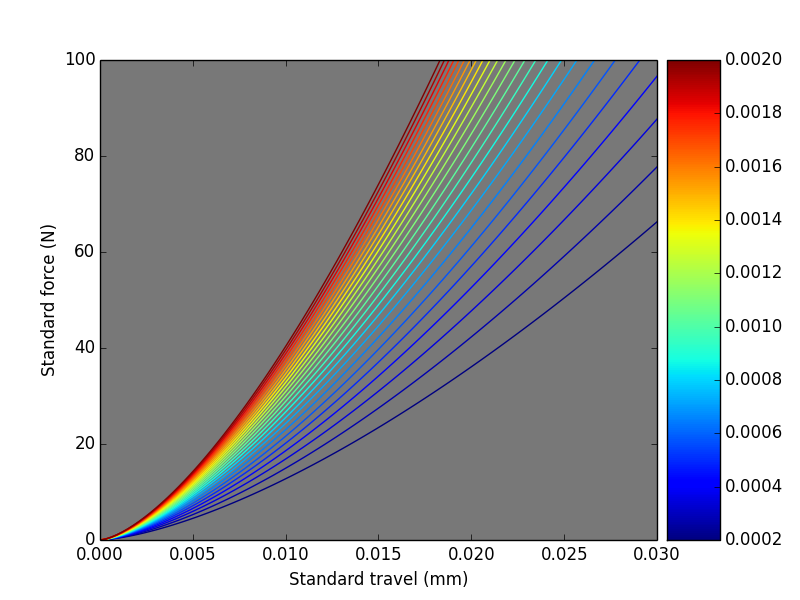
\includegraphics[width = \singleimagewidth]{chapters/figures/hertz-dp-dependence}
\caption{Hertzian responses of \lit pebbles compressed between platens. The colormap shows pebble diameters in \si{m}. The diameters span an order of magnitude from $d_p = \si{0.2 mm}$ to $d_p = \si{2 mm}$.}\label{fig:hertz-dp-dependence}
\end{figure}

\begin{figure}[!t]
\centering
    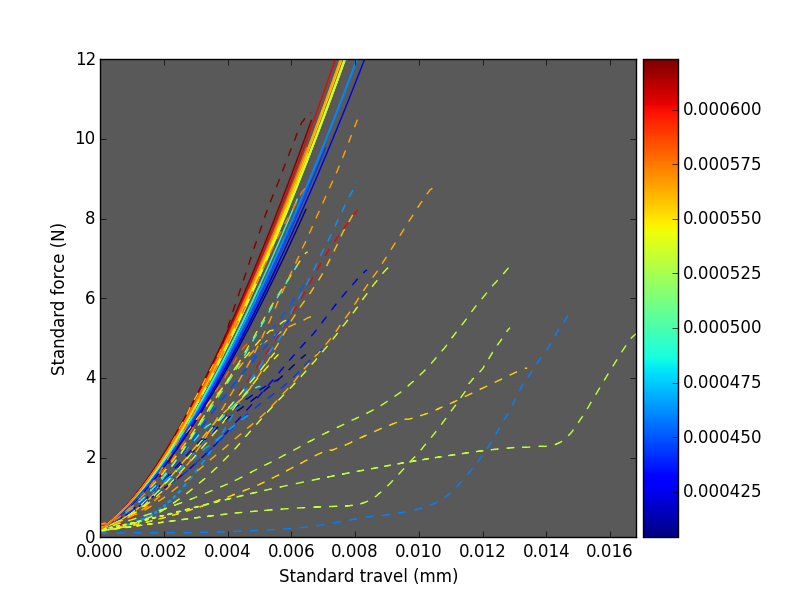
\includegraphics[width=\doubleimagewidth]{chapters/figures/fzk-data-w-ideal-hertz.png}
    \caption{Dashed lines are \lis pebbles of approximately \si{0.5 mm} diameter. Solid lines are the Hertzian (Eq.\ref{eq:contact-force}) responses based on each pebble's measured diameter.}
    \label{fig:fzk-exp-colormap}
\end{figure}

\begin{figure}
        \centering
        \begin{subfigure}[b]{\doubleimagewidth}
                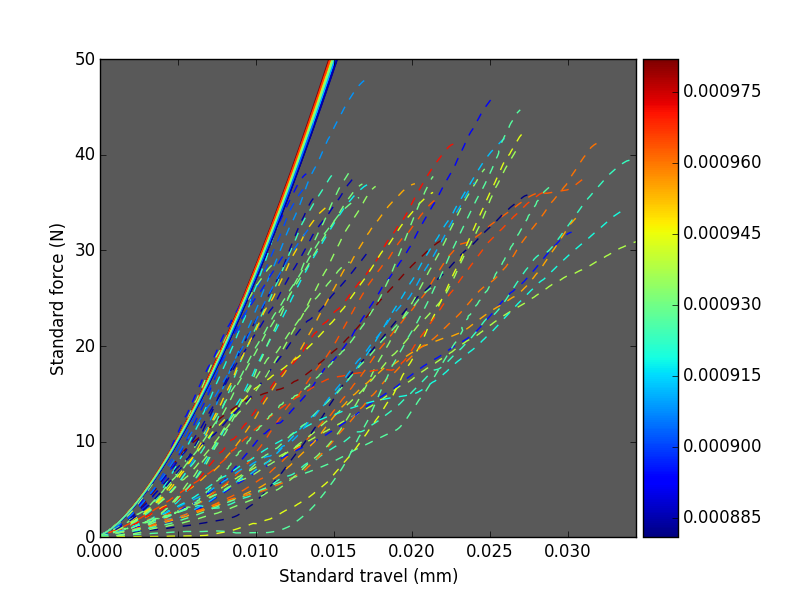
\includegraphics[width=\textwidth]{chapters/figures/nfri-1mm-data-w-ideal-hertz.png}
                \caption{$\bar{d}_p = 1$ mm}
                \label{fig:nfri-1-exp-colormap}
        \end{subfigure}
        ~
        \begin{subfigure}[b]{\doubleimagewidth}
                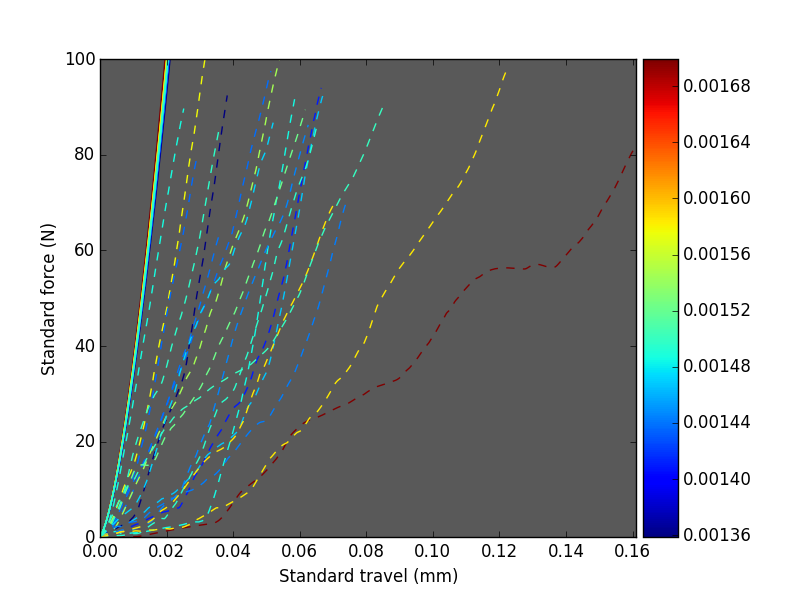
\includegraphics[width=\textwidth]{chapters/figures/nfri-1.5mm-data-w-ideal-hertz.png}
                \caption{$\bar{d}_p = 1.5$ mm}
                \label{fig:nfri-1.5-exp-colormap}
        \end{subfigure}
        \caption{Dashed lines are \lit pebbles. Solid lines are the Hertzian (Eq.\ref{eq:contact-force}) responses based on each pebble's measured diameter.}\label{fig:nfri-exp-curves}
\end{figure}


\begin{figure}[!t]
\centering
    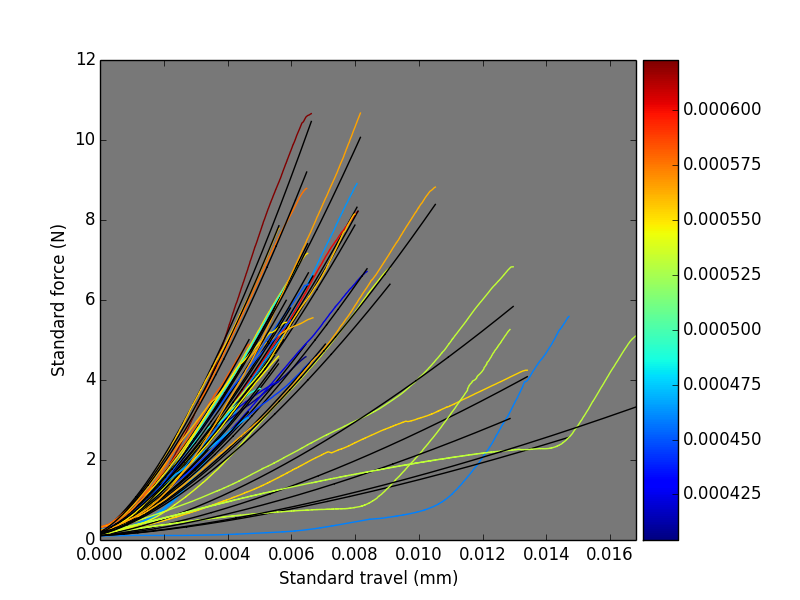
\includegraphics[width=\doubleimagewidth]{chapters/figures/fzk-hertz-colormap.png}
    \caption{Force-displacement curves for \lis pebbles (in color) along with their Hertzian fits (in black) calculated with each pebble having a unique Young's modulus.}
    \label{fig:fzk-exp-hertz}
\end{figure}

\begin{figure}
        \centering
        \begin{subfigure}[b]{\doubleimagewidth}
                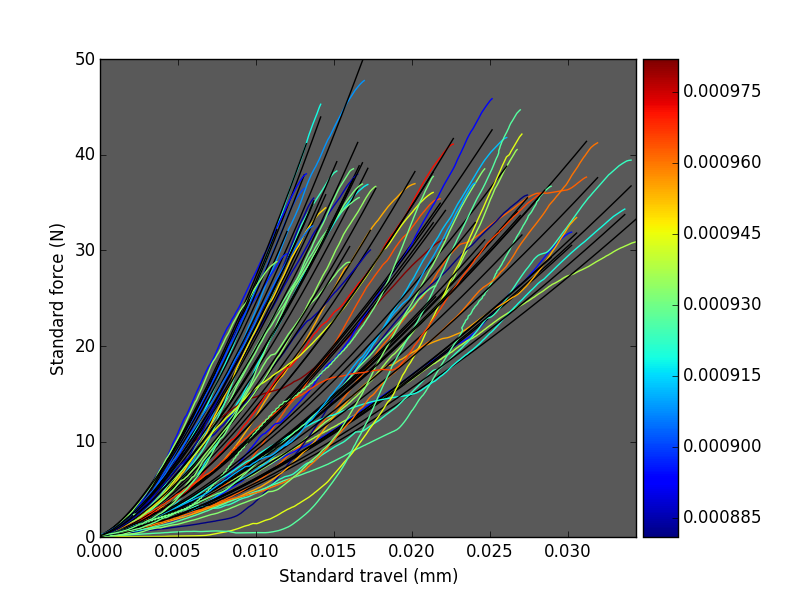
\includegraphics[width=\textwidth]{chapters/figures/nfri-1mm-hertz-colormap.png}
                \caption{$\bar{d}_p = 1$ mm}
                \label{fig:nfri-1-exp-hertz}
        \end{subfigure}
        ~
        \begin{subfigure}[b]{\doubleimagewidth}
                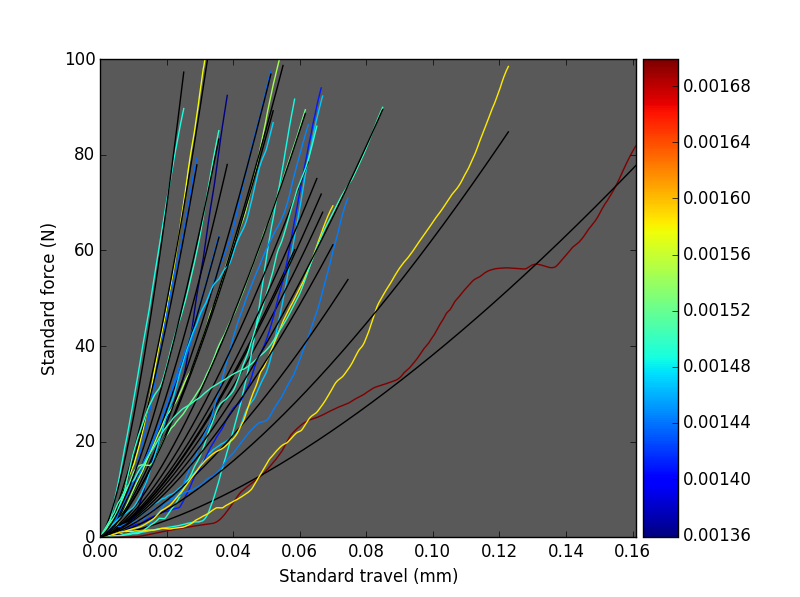
\includegraphics[width=\textwidth]{chapters/figures/nfri-1.5mm-hertz-colormap.png}
                \caption{$\bar{d}_p = 1.5$ mm}
                \label{fig:nfri-1.5-exp-hertz}
        \end{subfigure}
        \caption{Force-displacement curves for \lit pebbles (in color) along with their Hertzian fits (in black) calculated with each pebble having a unique Young's modulus.}\label{fig:nfri-exp-hertz}
\end{figure}

\begin{figure}[!t]
\centering
    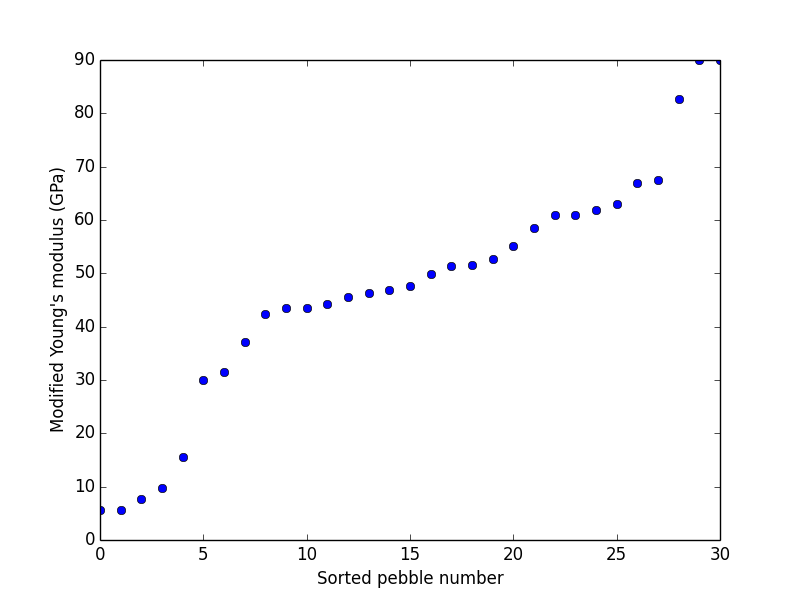
\includegraphics[width=\doubleimagewidth]{chapters/figures/fzk-E-plot.png}
    \caption{Distribution of modified Young's modulus for a batch of \lis pebbles. Most pebbles responded to compression with a Young's modulus well below the sintered pellet value of \si{90 GPa}.}
    \label{fig:fzk-E-plot}
\end{figure}

\begin{figure}
        \centering
        \begin{subfigure}[b]{\doubleimagewidth}
                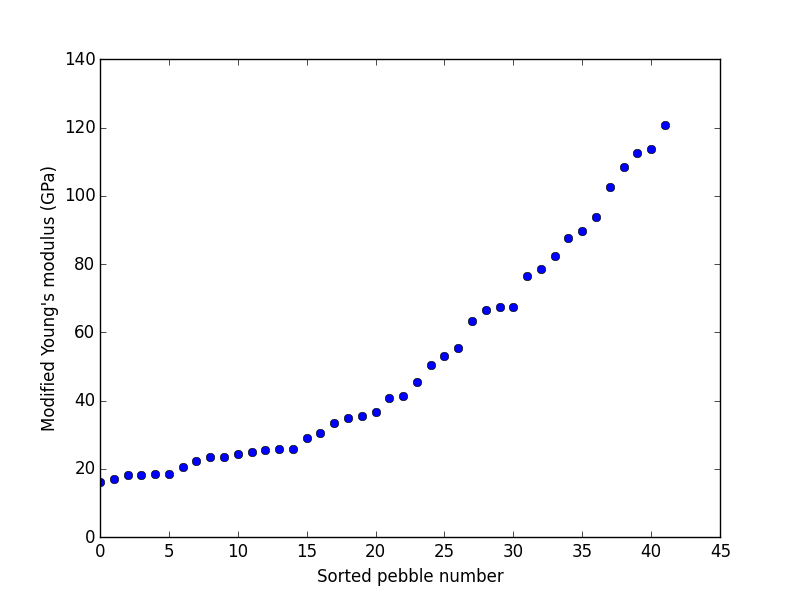
\includegraphics[width=\textwidth]{chapters/figures/nfri-1mm-E-plot.png}
                \caption{$\bar{d}_p = 1$ mm}
                \label{fig:nfri-1mm-E-plot}
        \end{subfigure}
        ~
        \begin{subfigure}[b]{\doubleimagewidth}
                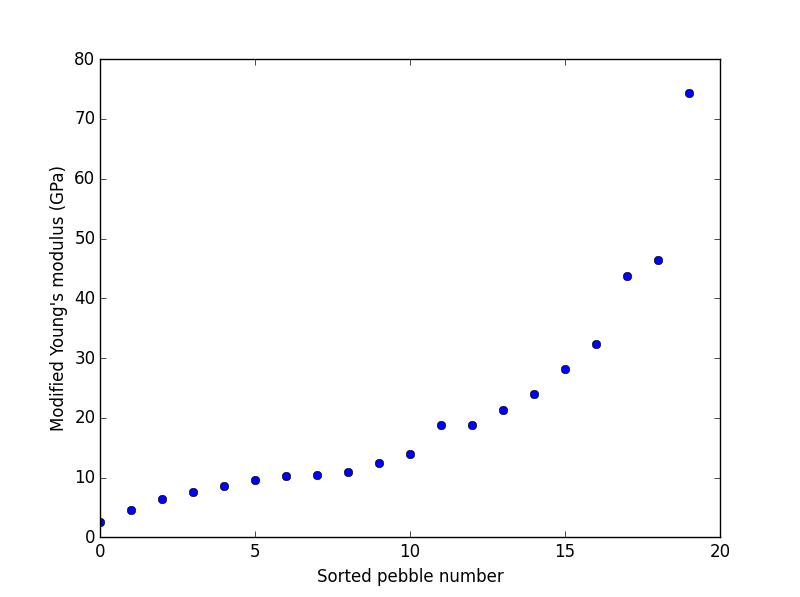
\includegraphics[width=\textwidth]{chapters/figures/nfri-1.5mm-E-plot.png}
                \caption{$\bar{d}_p = 1.5$ mm}
                \label{fig:nfri-1.5mm-E-plot}
        \end{subfigure}
        \caption{Distribution of modified Young's modulus for a batch of \lit pebbles. All pebbles responded to compression with a Young's modulus well below the sintered pellet value of \si{126 GPa}.}\label{fig:nfri-E-plot}
\end{figure}


\begin{figure}[!t]
\centering
    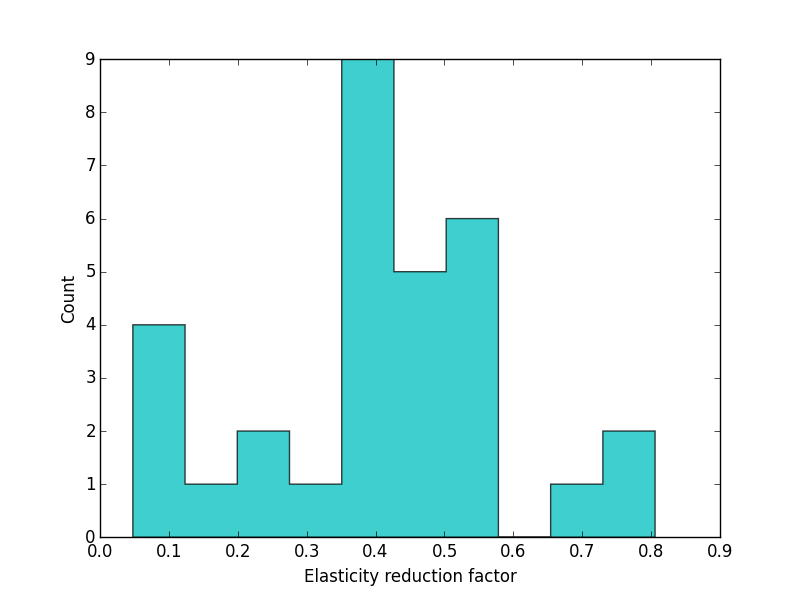
\includegraphics[width=\doubleimagewidth]{chapters/figures/fzk-kappa-histogram.png}
    \caption{Histogram of $\kappa$ for a batch of \lis pebbles. Most pebbles responded to compression with a Young's modulus well below the sintered pellet value of \si{90 GPa}.}
    \label{fig:fzk-kappa-hist}
\end{figure}

\begin{figure}
        \centering
        \begin{subfigure}[b]{\doubleimagewidth}
                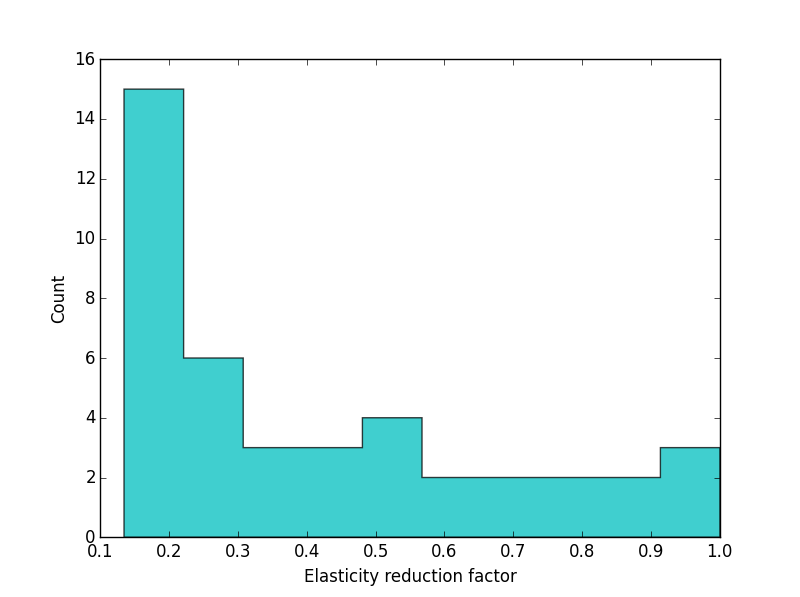
\includegraphics[width=\textwidth]{chapters/figures/nfri-1mm-kappa-histogram.png}
                \caption{$\bar{d}_p = 1$ mm}
                \label{fig:nfri-1mm-kappa-hist}
        \end{subfigure}
        ~
        \begin{subfigure}[b]{\doubleimagewidth}
                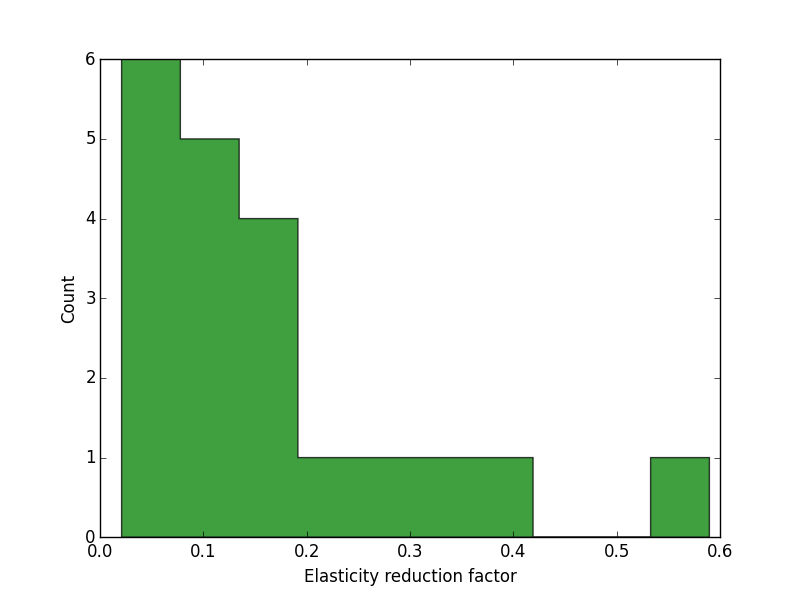
\includegraphics[width=\textwidth]{chapters/figures/nfri-1.5mm-kappa-histogram.png}
                \caption{$\bar{d}_p = 1.5$ mm}
                \label{fig:nfri-1.5mm-kappa-hist}
        \end{subfigure}
        \caption{Histogram of $\kappa$ for two batches of \lit pebbles. All pebbles responded to compression with a Young's modulus well below the sintered pellet value of \si{126 GPa}.}\label{fig:nfri-kappa-hist}
\end{figure}


\begin{figure}[!ht]
\centering
    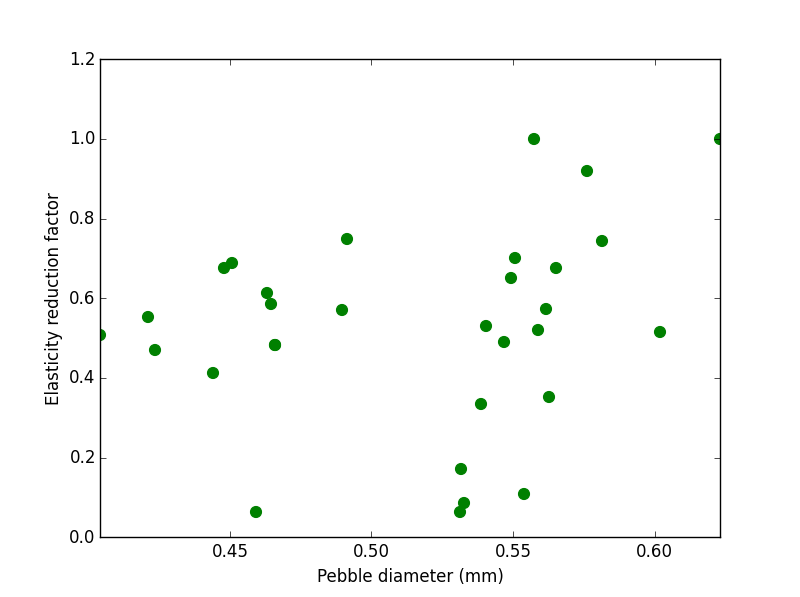
\includegraphics[width=\doubleimagewidth]{chapters/figures/fzk-kappa-dp-scatter.png}
    \caption{Scatter of $\kappa$ against pebble diameter for a batch of \lis pebbles showing almost no relationship between apparent stiffness and diameter.}
    \label{fig:fzk-kappa-dp-scatter}
\end{figure}

\begin{figure}
        \centering
        \begin{subfigure}[b]{\doubleimagewidth}
                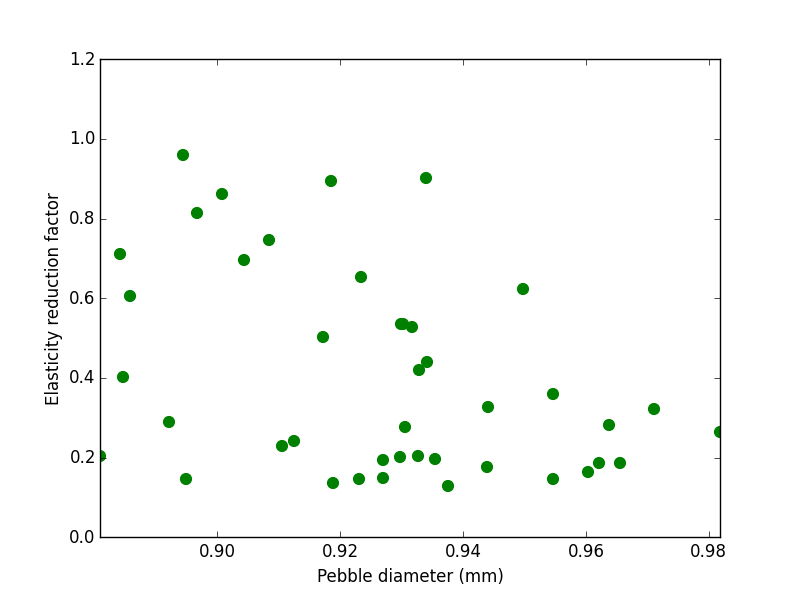
\includegraphics[width=\textwidth]{chapters/figures/nfri-1mm-kappa-dp-scatter.png}
                \caption{$\bar{d}_p = 1$ mm}
                \label{fig:nfri-1mm-kappa-dp-scatter}
        \end{subfigure}
        ~
        \begin{subfigure}[b]{\doubleimagewidth}
                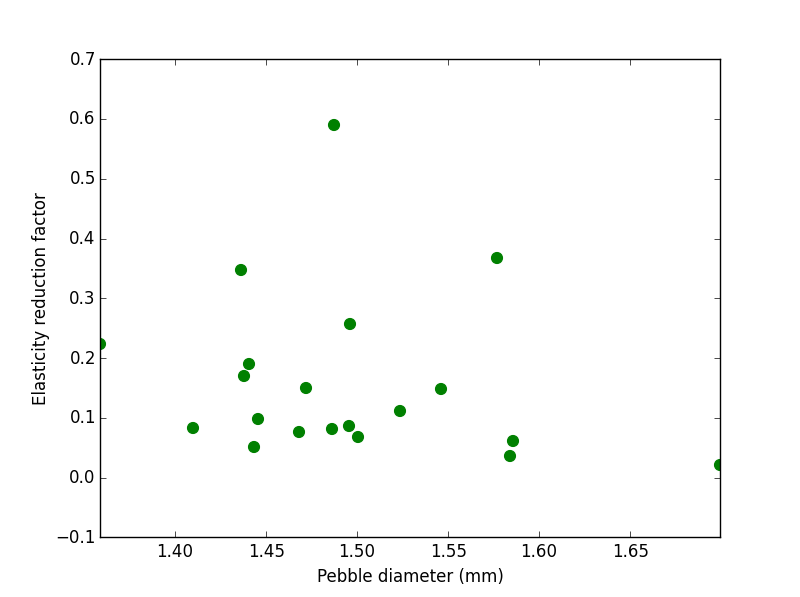
\includegraphics[width=\textwidth]{chapters/figures/nfri-1.5mm-kappa-dp-scatter.png}
                \caption{$\bar{d}_p = 1.5$ mm}
                \label{fig:nfri-1.5mm-kappa-dp-scatter}
        \end{subfigure}
        \caption{Scatter of $\kappa$ against pebble diameter for two batches of \lit pebbles showing almost no relationship between apparent stiffness and diameter.}\label{fig:nfri-kappa-dp-scatter}
\end{figure}






The Young's modulus and Poisson ratio of the test stand are known values that do not vary between pebble experiments. Similarly, in the application of Hertz theory, we also assume the Young's modulus and Poisson ratio of the ceramic is also a known, constant value. In that case, for any given pebble diameter, the term inside $[\,]$ is composed of entirely of constants for any given pebble; there is therefore a single force-travel response possible based on $s$. Using the material properties given in Ref.~\cite{Gierszewski1998} for \lit, we plot a set of parametric curves based on diameter over a range of travel. The properties we have used for the nickel-alloy anvil of our test stand and \lit are given in Table~\ref{tab:hertz-dp-study-props}. The curves are given in Fig.~\ref{fig:hertz-dp-dependence}.

\begin {table}[htp] %
\caption{Material properties used for \lit and nickel-alloy platen}
\label {tab:hertz-dp-study-props} \centering %
\begin {tabular}{ cccccc }
\toprule %
$E_\text{peb}$      &     $\nu_\text{peb}$  &   $E_\text{stand}$        &     $\nu_\text{stand}$    \\
(GPa)           &                   &   (GPa)               &                   \\\toprule
126             &   0.24                &   220                 &   0.27                \\\bottomrule
\end{tabular}
\end{table}

Figure~\ref{fig:hertz-dp-dependence} shows that, for a given pebble diameter, there is a  is strictly obeying Hertz theory, there is only a single force-displacement curve it can follow. However, when experiments are performed on single pebbles of \lis we see responses in the dashed lines of Fig.~\ref{fig:fzk-exp-colormap}. Similarly for the dashed lines of \lit in Fig.~\ref{fig:nfri-exp-curves}.

Contrary to the diameter dependence seen in Fig.~\ref{fig:hertz-dp-dependence}, the curves of Figs.~\ref{fig:fzk-exp-colormap},~\ref{fig:nfri-exp-curves} do not demonstrate any relationship between diameter and force. For comparison, the solid lines on the figures for each ceramic show the predicted Hertzian response as calculated by Eq.~\ref{eq:contact-force} based on the measured diameter of each pebble. For both the \lis and \lit pebbles, there are very few pebbles that show a measured force-travel response that is similar to the Hertzian prediction based on the material properties reported in literature. We conclude that variations in pebble diameter can not alone account for the variations in the force curves measured for the pebbles in our experiments. %The most reasonable source for variation is in the Young's modulus of pebbles in a batch. Such a conclusion is important for implementation of Hertz theory in DEM algorithms.

We hypothesize that variation in measured curves is due to each pebble having Young's modulii that diverge from the values measured from sintered blocks as reported in literature. Therefore each pebble displays a different apparent Young's modulus in the single pebble experiments. The apparent Young's modulus of each pebble is rooted in the manufacture of the pebbles which yields pebbles with slightly different internal structures. The differences in internal structure then cause the pebble to behave with different stiffnesses than the value expected from measurements of sintered pellets of lithium ceramics. In fact, the solid lines in Figs.~\ref{fig:fzk-exp-colormap},~\ref{fig:nfri-exp-curves}, as calculated from the measurements of sintered pellets, appear to be an upper limit to the pebbles. Therefore we consider pebbles will emerge with values less than the value from literature, $E_\text{lit}$ by some factor. To quantify the deviation of each pebble's $E_\text{peb}$ from the sintered pellet, we introduce a $\kappa$ factor, which we define as the elasticity reduction factor:

\begin{equation}
\kappa = \frac{E_\text{peb}}{E_\text{lit}}
\end{equation}
where
\[
\kappa \in [0,1]
\]

If each pebble has a unique $\kappa$ value, it would quantify the spread in elastic responses seen in the experiments. We find the value by assuming that the pebbles are, in fact, behaving in a Hertzian manner and we can fit the Hertzian to our experimental measurements. This allows us to back-out a $\kappa$ value, or in other words the unique $E_\text{peb}$ of that pebble. We take the sintered pebble value of Young's modulus for \lis to be $E_\text{lit} = \si{90 GPa}$ and the value for \lit to be $E_\text{lit}= \si{124 GPa}$. Then we iterate over all values of $k\in[0,1]$ and compare the Hertzian response to that pebbles force-displacement curve. At each iteration, the L2-norm of the difference between Hertzian and experimental curves is used as the `error'. The L2 norm, $A$ for a given array, $a$ is 

\begin{equation}
||A||_F = \left[\sum_{i,j}\textrm{abs}(a_{i,j})^2\right]^{1/2}
\end{equation}

This is a convenient way to compare the error at every point along the force-displacement curves. When the error is minimized, the elasticity reduction value corresponding the minimum is recorded for that pebble. In The Hertzian curves (in black) for each pebble are plotted in green against the experimental curves in Figs.~\ref{fig:fzk-exp-hertz},~\ref{fig:nfri-exp-hertz}. 



Many of the curves for \lis in Fig.~\ref{fig:fzk-exp-hertz} seem to be fit well with a Hertzian curve with modified Young's modulus. The value of Young's modulus found for each pebble is plotted in Fig.~\ref{fig:fzk-E-plot}. The Young's modulus of pebble numbers 0 to 4 are the very soft pebbles seen with very low forces on Fig.~\ref{fig:fzk-exp-hertz}. The majority of pebbles, however, behave with a Young's modulus between 30 and 70 \si{GPa}. On the upper end, a few pebbles acted very similar to their sintered pellet counterpart with approximate value of \si{90 GPa}. 

The two batches of \lit pebbles we analyzed (Fig.~\ref{fig:nfri-exp-hertz}) are similarly fit well to different Hertzian curves. The apparent Young's modulii of the \lit pebbles are given in Fig.~\ref{fig:nfri-E-plot}. These \lit pebbles have a large distribution of stiffness, from between 20 to 120~GPa for the 1~mm pebbles and roughly 2 to 80~GPa for the 1.5~mm pebbles.


A histogram of the $\kappa$ factor for this batch of \lis pebbles is given in Fig.~\ref{fig:fzk-kappa-hist}. For the \lis pebbles, the histogram resembles a normal distribution but for the large spike in pebbles with very small $\kappa$. When we look back to the force-travel plots of Fig.~\ref{fig:fzk-exp-colormap}, the four softest pebbles show similar trends of long, relatively flat responses to travel before reaching a point where there is a sharp increase in the $F-s$ slope. In the experiments, the flat sections of the curve occurred when the pebbles in the anvil were not perfectly spherical and rotated slightly under the application of a load. Once the pebbles rotated into a flat spot that could take a normal load without any angular moment, the force increased quickly under further travel. In light of this, it is unreasonable to consider their $\kappa$ values as representing their true stiffness. Neglecting the four outliers in the histogram of Fig.~\ref{fig:fzk-kappa-hist}, we are then left with a distribution much more closely resembling a normal probability distribution.

The histograms for the two batches of \lit are given in Fig.~\ref{fig:nfri-kappa-hist}. The distributions for both batches of \lit pebbles more closely resemble Snedecor's F distribution with many pebbles behaving with a very small $\kappa$.

In Figs.~\ref{fig:fzk-kappa-dp-scatter} and~\ref{fig:nfri-kappa-dp-scatter} we see scatter plots of the pebble diameters and $\kappa$ values for the different batches of lithium ceramic pebbles. A Pearson Correlation value was calculated for each of the batches to find a relationship between diameter and $\kappa$. For the \lis pebbles, we find $R = 0.198$ which is a weak positive correlation. For the \lit pebbles we have $R = -0.385$ for $\bar{d}_p = 1$~mm and $R = -0.201$ for $\bar{d}_p = 1.5$~mm. Both of these are weakly negatively correlated. 

The implications of these results are that the Young's modulus traditionally used in DEM simulations for ceramic pebble beds in solid breeders is incorrect. In \cref{sec:dem-studies-youngs-modulus}, we will introduce $\kappa$, the elasticity reduction factor, into our DEM simulations. Numerical recreations of the probability distribution curves will be used to apply $\kappa$ to pebbles in the ensemble. From the weak correlations between diameter and $\kappa$, we are free to ignore any diameter dependence when assigning $\kappa$ values in the DEM framework. In the module where we assign Young's modulus to the particles in the ensemble will apply the distribution in a random fashion.

\FloatBarrier
\subsection{Translating Experimental Results to Pebble Bed Interactions}\label{sec:theoryStrainEnergy}

It is impractical, if not impossible, to accurately measure the contact forces between all the pebbles in a densely-packed, three-dimensional ensemble. In investigating the probability of pebbles becoming damaged (i.e. crushed or cracked) in a packed bed, we therefore rely on the combined information gained from indirect measurements of the entire pebble bed, crush experiments of individual pebbles, and the predictive capabilities of DEM simulations. In this study we look at the results of individual pebble crush experiments and create a metric to link the data to the contact forces measured in DEM to help predict when pebbles in the ensemble will become damaged.

\subsubsection{Experimental Measurements of Strain Energy}
\begin{figure}[!t]
\centering
    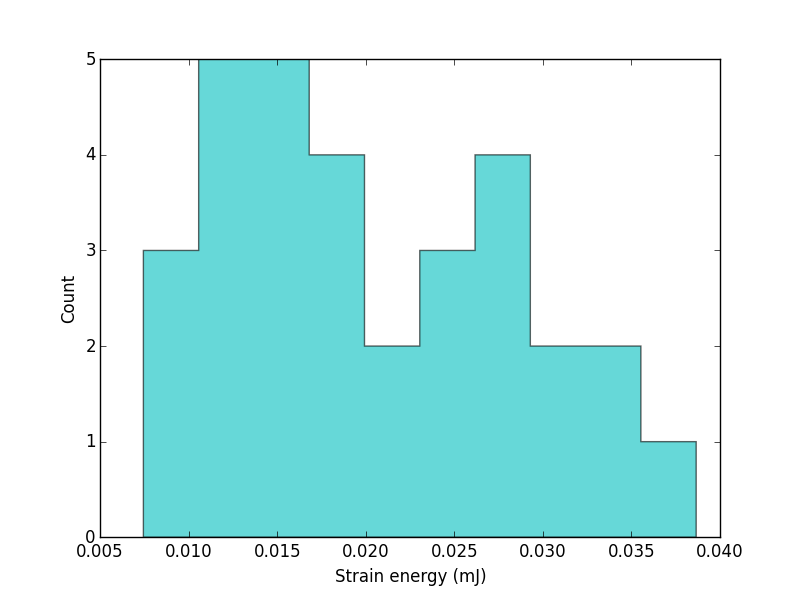
\includegraphics[width=\doubleimagewidth]{chapters/figures/fzk-w-histogram.png}
    \caption{Histogram of the absorbed strain energy at the moment of crushing for \lis pebbles as measured in single pebble crush experiments.}
    \label{fig:fzk-w-hist}
\end{figure}

\begin{figure}
        \centering
        \begin{subfigure}[b]{\doubleimagewidth}
                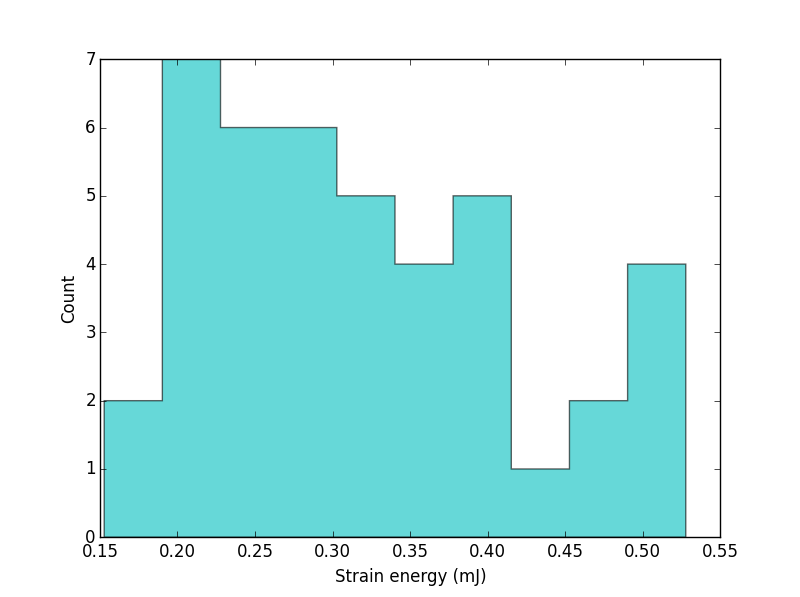
\includegraphics[width=\textwidth]{chapters/figures/nfri-1mm-w-histogram.png}
                \caption{$\bar{d}_p = 1$ mm}
                \label{fig:nfri-1-w-hist}
        \end{subfigure}
        ~
        \begin{subfigure}[b]{\doubleimagewidth}
                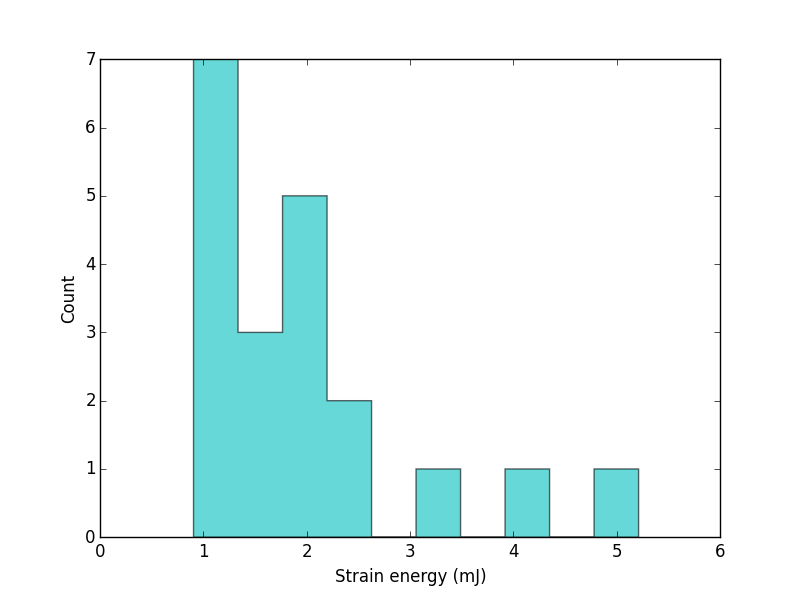
\includegraphics[width=\textwidth]{chapters/figures/nfri-1.5mm-w-histogram.png}
                \caption{$\bar{d}_p = 1.5$ mm}
                \label{fig:nfri-1.5-w-hist}
        \end{subfigure}
        \caption{Histogram of the absorbed strain energy at the moment of crushing for \lit pebbles as measured in single pebble crush experiments.}\label{fig:nfri-w-hist}
\end{figure}

The normal force between two elastic objects is a function of the material properties of the interacting objects (see Eq.~\ref{eq:hertz-normal-force}). We cannot, therefore, directly compare the forces between pebble-test stand with pebble-pebble in an ensemble. An approached used by some solid breeder researchers is to relate the absorbed strain energy of the pebble\cite{Zhao2013,Annabattula2012a}. We integrate the Hertzian force along the overlap to find the strain energy, $W_\epsilon$, of that contact. 

\begin{equation}\label{eq:strain-energy-integral}
	W_\epsilon = \int_0^{\delta_c}\!F_n(\delta')\,\mathrm{d}\delta'
\end{equation}
where the upper limit of the integration is the critical overlap $\delta_c$. Inserting Eq.~\ref{eq:hertz-normal-force} into Eq.~\ref{eq:strain-energy-integral},
\begin{align}
	W_\epsilon& = \int_0^{\delta_c}\!  \frac{4}{3}E^*\sqrt{R^*}\,\delta'^{3/2} \,\mathrm{d}\delta' \\
	%W_\epsilon & = \frac{4}{3}E^*\sqrt{R^*} \left[\frac{2}{5}\,{\delta_c}^{5/2}\right] \\
	W_\epsilon & = \frac{8}{15}E^*\sqrt{R^*}\, {\delta_c}^{5/2}
\end{align}

We will call the strain energy of the pebble compressed between platens as the lab strain energy, $W_{\epsilon,L}$. In pebble crushing experiments, we record the strain energy absorbed up to the point of crushing, the data for \lis and \lit pebbles are given in Figs.~\ref{fig:fzk-w-hist} and~\ref{fig:nfri-w-hist}, respectively. Then the strain energy of two particles in contact will be $W_{\epsilon,B}$. The assumption we make is that, if each contact interaction is integrated to the proper critical overlap, the strain energies will be equal at that contact.

\begin{equation}
	W_{\epsilon,L} = W_{\epsilon,B} = \frac{8}{15}E_B^*\sqrt{R_B^*}\, {\delta_{c,B}}^{5/2}
\end{equation}

We solve for the interacting pebble bed overlap as a function of the lab strain energy as

\begin{equation}
	\delta_{c,B} = \left[\frac{15W_{\epsilon,L}}{8E_B^*\sqrt{R_B^*}}\right]^{2/5}
\end{equation}

This overlap can be reinserted to the Hertz force of Eq.~\ref{eq:hertz-normal-force} to find the critical force (crush force) of the interacting particles as a function of the critical strain energy of the lab. Doing this, we find,
\begin{equation}\label{eq:peb_hertz}
	F_{c,B} = C{E_B^*}^{2/5}{R_B^*}^{1/5}W_{\epsilon,L}^{3/5}
\end{equation}
where $C = \frac{4}{3}\left(\frac{15}{8}\right)^{3/5}$.

Equation~\ref{eq:peb_hertz} is a generic translation between lab materials and packed bed materials. We will use the equation as the basis for our pebble crushing prediction in DEM simulations.





% FROM SOFT PAPER
\subsubsection{Calculating Critical Strain Energy}
With the rise of micro-mechanical tools and computing power, attempting to predict when ceramic pebbles will crush in an ensemble, based on inter-particle contact forces, has received considerable attention. In this section we will review literature studying granular crushing.

Probability and statistics were applied to the study of packed beds of brittle grains by Marketos and Bolton\cite{Marketos2007}. The fundamental assumption in their predictive method was the independence of crushing events. They used their model to predict the initiation of crushing as well as the evolution of the packing after crushing. They created somewhat arbitrary probability distributions of the strength of their granular particles,
\begin{equation}
	h(\Phi) = \frac{0.0395}{\sqrt{\Phi}}
\end{equation}
where $\Phi$ is a characteristic strength parameter falling between 160 and 640~N. The form of their distribution was based on single crushing tests on quartz particles from Nakata\etal.

A common alternative distribution is to use a form first proposed by Weibull for a material under uniform stress\cite{Kwok2013,Zhao2011,nakata1999probabilistic,Zhao2013,Pitchumani2004}. The form, as written by Zhao\etal~is,
\begin{equation}
	P_s = 1 - \exp\left[-\left(\frac{W_c}{W_\text{mat}}\right)^m\right]
\end{equation}
where $W_c$ is the energy absorbed by the pebble and $W_\text{mat}$ and $m$ characterize the material. An important note is how to calculate the critical strain energy for the pebble. Refs.~\cite{Marketos2007} and \cite{Zhao2011} note the necessity to consider the coordination number dependence on total strain energy. In other words, the total strain energy is the cumulative total of strain energy at every contact. Zhao\etal~give strain as
\begin{equation}
	W_c = \sum_{i=1}^{Z_i}\left(\frac{9}{80 R_{ij}^*}\right)^{1/3} \left(\frac{1}{E_{ij}^*}\right)^{2/3} F_{n,ij}^{5/3}
\end{equation}
where $Z$ is the coordination number of pebble $i$. 

However, Russell\etal, analyzed ideal granular assemblies for which they could find analytical solutions to stress distributions inside of pebbles.\cite{Russell2009} In their work, failure of a granular particle initiates at the location of maximum of the stress invariant ratios. In the contact of elastic spheres, the stress fields near the contact areas are highly localized. Because of the highly localized effects, Russell\etal~find that in granular assemblies the contributions to failure initiation are not additive. They discovered that the initiation of failure is always located adjacent to the largest force irrespective of the material properties or geometric size of the pebbles in an ensemble. Russell\etal\cite{Russell2009} conclude: the largest contact force acting upon a particle is the primary agent driving the damage of the individual. Based upon the failure criterion developed for brittle materials, crushing of an individual does not directly depend upon the presence or magnitude of any lesser contact forces acting on the particle or the material properties of the particle. Although their results were obtained for idealized assemblies, the results are generally true for any situation where multiple contact forces are present.

\begin{figure}[!t]
\centering
    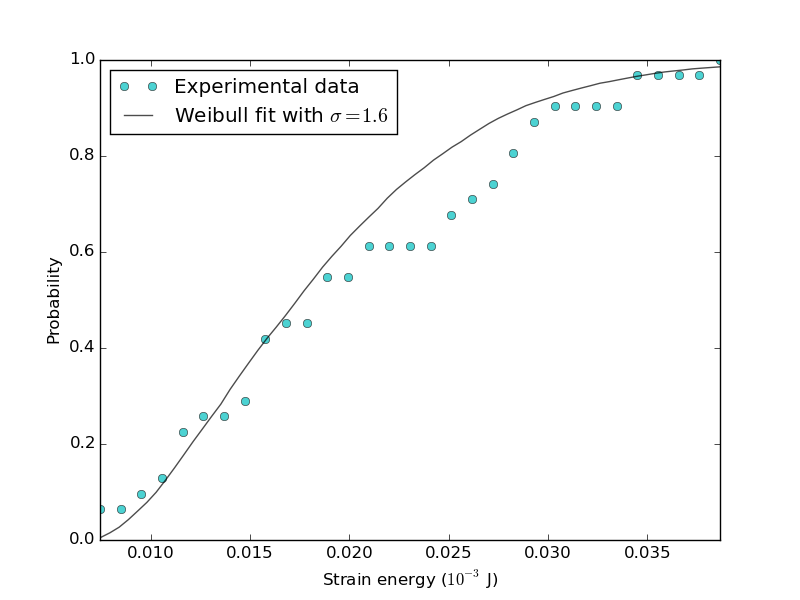
\includegraphics[width=\doubleimagewidth]{chapters/figures/fzk-w-cdf-fit.png}
    \caption{Fitting the strain energy with a Weibull distribution with shape parameter specific for the \lis pebbles.}
    \label{fig:fzk-w-cdf}
\end{figure}

\begin{figure}
        \centering
        \begin{subfigure}[b]{\doubleimagewidth}
                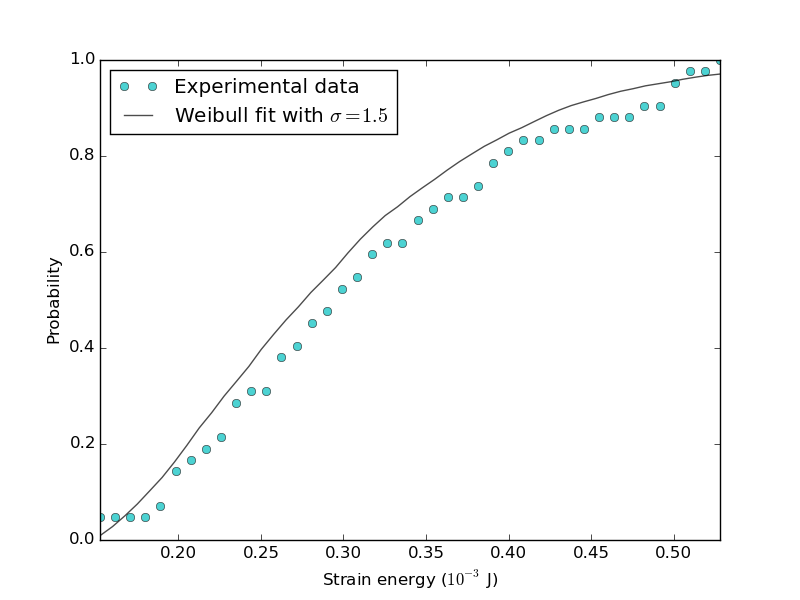
\includegraphics[width=\textwidth]{chapters/figures/nfri-1mm-w-cdf-fit.png}
                \caption{$\bar{d}_p = 1$ mm}
                \label{fig:nfri-1-w-cdf}
        \end{subfigure}
        ~
        \begin{subfigure}[b]{\doubleimagewidth}
                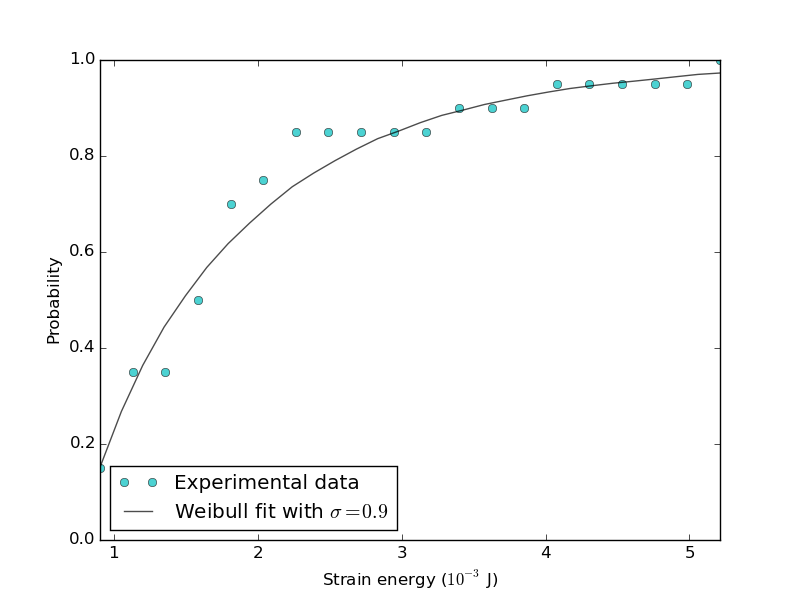
\includegraphics[width=\textwidth]{chapters/figures/nfri-1.5mm-w-cdf-fit.png}
                \caption{$\bar{d}_p = 1.5$ mm}
                \label{fig:nfri-1.5-w-cdf}
        \end{subfigure}
        \caption{Fitting the strain energy with a Weibull distribution with shape parameter specific for the two batches of \lit pebbles.}\label{fig:nfri-w-cdf}
\end{figure}

Based on the compelling arguments of Russell\etal, we will define our critical force as the maximum contact force on the pebble in our assembly,
\begin{equation}
	F_{c} = \max F_{n,ij}
\end{equation}

Then we can say a pebble is crushed when the force on the pebble in the bed is greater than the critical bed force defined from Eq.~\ref{eq:peb_hertz},

\begin{equation}\label{eq:crush-predict}
  F_{c} > F_{c,B} = \frac{4}{3}\left(\frac{15}{8}\right)^{3/5}{E_B^*}^{2/5}{R_B^*}^{1/5}W_{\epsilon,L}^{3/5}
\end{equation}

In the implementation into DEM, the probabilistic features appear naturally in this formulation from the measured probability distribution of $W_{\epsilon,L}$. In the experiments on crushing individual pebbles, the critical strain energy is measured strain energy at the point of crushing. This value follows a probability distribution and therefore imparts a distribution shape to the $F_{c,B}$ prediction. Cumulative distribution functions are generated for the strain energy data (see Figs.~\ref{fig:nfri-w-hist} and~\ref{fig:nfri-w-hist}). From that data, we fit Weibull distribution curves, of the form
\begin{equation}
	\Xi = \lambda\left[-\ln(W_\epsilon)\right]^{1/\sigma}
\end{equation}
where the shape parameter, $\sigma$, is fit to the specific curve of each set of experimental data and the second parameter, $\lambda$ is
\[
\lambda = \bar{W}_\epsilon - \min W_\epsilon
\]

In Figs.~\ref{fig:fzk-w-cdf} and~\ref{fig:nfri-w-cdf} we show the experimental data and the Weibull fits specific to the ceramic material and batch. The Weibull distribution functions will be used again when we generate strength parameters to assign to pebbles in the discrete element simulations of pebble crushing, addressed in \cref{sec:failure-study}.







